\documentclass{beamer}
\usepackage[english]{babel}
\usepackage[utf8]{inputenc}
\usepackage{times}
\usepackage[T1]{fontenc}
%\usepackage{subfigure}
%\usepackage{wrapfig}
\usepackage{float}
\usepackage{ctable}
\usepackage{colortbl}
\usepackage{pgfpages}
\usepackage{cancel}
\usepackage{minted}

\mode<presentation>
{
  \usetheme{Singapore}
  \usecolortheme{rose}
  %\usefonttheme[onlylarge]{structurebold}
  %\setbeamerfont*{frametitle}{size=\normalsize,series=\bfseries}
  % or ...
  \setbeamercovered{transparent}
  % or whatever (possibly just delete it)
  \setbeamertemplate{navigation symbols}{}
  \setbeamertemplate{note page}[plain]
  %\logo{\includegraphics[width=1.2 cm]{figuras/logo_ufes}}
  \setbeamertemplate{footline}{\hfill\scriptsize{\vspace*{5pt}\color{gray}{\insertframenumber}\hspace*{5pt}}} 
  %\setbeamertemplate{footline}{%
  %\leavevmode%
  %\hbox{%
  %\begin{beamercolorbox}[wd=.5\paperwidth,ht=2.25ex,dp=1ex,right]{author in
  %    head/foot}%
  %    \usebeamerfont{author in head/foot}\insertshortauthor \hspace{.5cm}
  %    (\insertshortinstitute) \hspace{.5cm}
  %\end{beamercolorbox}%

  %\begin{beamercolorbox}[wd=.5\paperwidth,ht=2.25ex,dp=1ex,left]{title in
  %    head/foot}%
  %    \usebeamerfont{title in head/foot} \hspace{.5cm}\insertshorttitle
  %\end{beamercolorbox}}%
  %\vskip0pt%
  %}
}

% Define o tema da apresentacao (soh fica guardado nas informacoes do pdf)
\subject{SVM optimization}
% Delete this, if you do not want the table of contents to pop up at
% the beginning of each subsection:
% \AtBeginSubsection[]
% {
%   \begin{frame}<beamer>{Sumário}
%     \tableofcontents[currentsection,currentsubsection]
%   \end{frame}
% }
% \AtBeginSection[]
% {
%   \begin{frame}<beamer>{Sumário}
%     \tableofcontents[currentsection]
%   \end{frame}
% }
%\setbeameroption{show notes}
%\setbeameroption{show notes on second screen=right}
%============================================================================================

\title{Linear Hard Margin SVM for Classification and Pattern Recognition}


\author[Boechat A.A.]
{ 
    André Ambrósio Boechat
}
\institute[UFSC]{Departamento de Automação e Sistemas\\Universidade Federal de Santa
Catarina}

%Programa de Pós-Graduação em Eng. de Automação e Sistemas\\Universidade Federal
%de Santa Catarina
%}

% Se comentar a linha abaixo, ira aparecer a data quando foi compilada a apresentacao
\date{Florianópolis, October 2012}

\setbeamercolor{postit}{fg=black,bg=block body.fg!75!black!10!bg}
% =========================================================================================
\begin{document}

\begin{frame}
    \titlepage
    \thispagestyle{empty}

\end{frame}


\begin{frame}{Contents}
    \tableofcontents[]
\end{frame}

\section{Introduction}

\begin{frame}{Data-Driven Models}

    \begin{itemize}
        %% Some applications
        \item Regression, pattern recognition, \alert{classification}
            \vspace{.5cm}
            \begin{block}{Classification}
                Separation of samples in different \alert{classes}, trying to find a
                possible \alert{decision boundary}.
            \end{block}
            \vspace{.5cm}
        %% Some similar techniques
        \item Well-known classifiers
            \begin{itemize}
                \item Naive Bayes classifier
                \item Logistic regression
                \item Artificial Neural networks (ANN)
                \item Support Vector Machines (SVM)
            \end{itemize}
    \end{itemize}
\end{frame}


\begin{frame}{Support Vector Machines}
    \begin{itemize}
        \item The foundations were recently developed (Vapnik, 1995)
        %% Because of risk minimization strategy, some authors say that: 
        \item Greater ability to generalize than ANN
        \item Many possible formulations
            \begin{itemize}
                \item \alert{linear}
                \item nonlinear
                \item regression
            \end{itemize}
        %% One the main properties:
        \item \alert{Large margin} classifier
    \end{itemize}

    %% FILE Ryan M. Rifkin
    \begin{figure}[!htb]
        \centering
        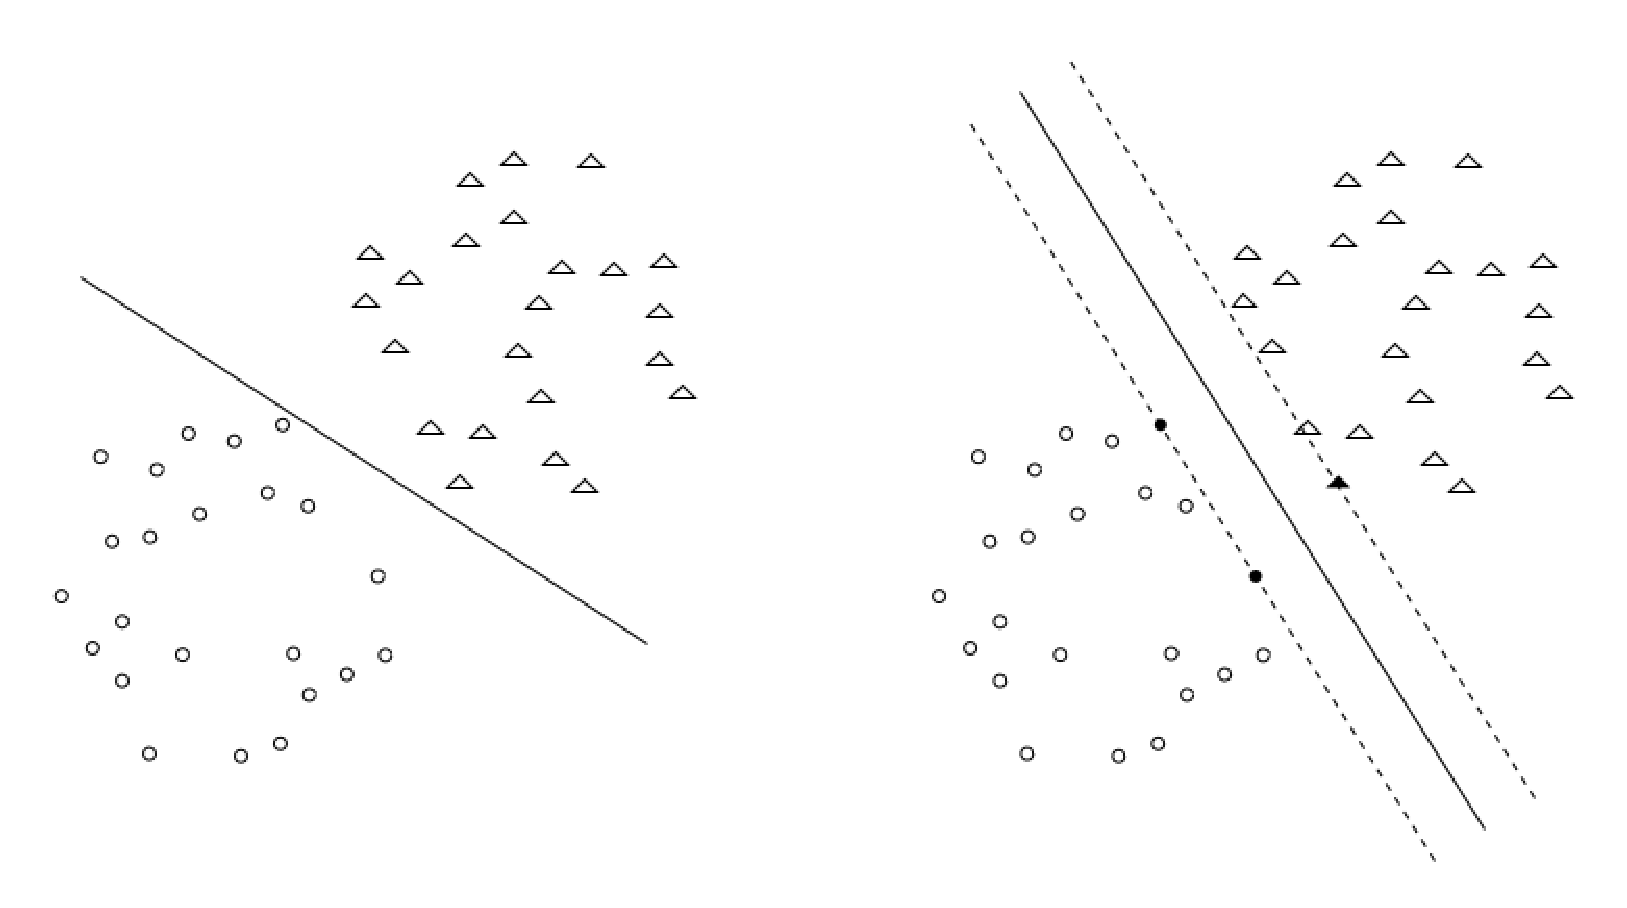
\includegraphics[width=.8\textwidth]{figures/large_margin.eps}
    \end{figure}
\end{frame}


\section{Linear SVM Formulation}

\subsection{Problem Formulation}

\begin{frame}{Geometrical Interpretation~\cite{Burges1998}}
    Training data composed of $m$ samples
    $$
    \begin{array}{l}
        \left\{\mathbf{x}^{(i)}, y^{(i)}\right\}, \quad i = 1, \cdots, m\\[.2cm]
                %% Features 
        \mathbf{x}^{(i)} \in \mathbb{R}^n\\[.2cm]
                %% Labels
        y^{(i)} \in \{-1, 1\}
    \end{array}
    $$

    We want to find a $f(\mathbf{x})$ which determines a separating hyperplane
    \begin{equation}
        %% w is normal to the hyperplane
        \mathbf{w}^T \mathbf{x} + b = 0
        \label{eq:f_hyperplane}
    \end{equation}
    %% Hyperplane distance from origin
    %$$\frac{|b|}{||\mathbf{w}||}$$

    For the linearly separable case, a hyperplane with the largest margin must obey the
    following constraints
    %
    \begin{equation}
        \begin{array}{ll}
            \mathbf{w}^T \mathbf{x}^{(i)} + b \ge 1, & \quad \mbox{for} \quad y^{(i)} =
            1\\[.2cm]
            \mathbf{w}^T \mathbf{x}^{(i)} + b \le -1, & \quad \mbox{for} \quad y^{(i)} = -1
        \end{array}
        \label{eq:orig_constraints}
    \end{equation}
\end{frame}

\begin{frame}{Hyperplane with the Largest Margin}
    \begin{figure}[!htb]
        \centering
        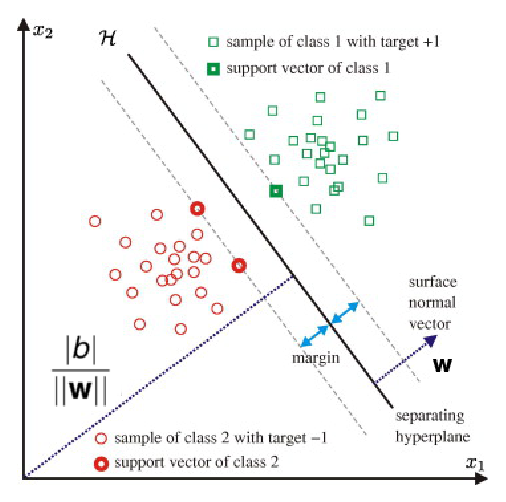
\includegraphics[width=.6\textwidth]{figures/svm_hyperplane2.eps}
        \caption{Adapted from \cite{Fisch20103381}}
    \end{figure}
\end{frame}

\begin{frame}
    The support hyperplanes given by the constraints of Eq. \eqref{eq:orig_constraints}
    are
    %
    \begin{equation}
        \begin{array}{l}
            \mathcal{H}_1: \quad \mathbf{w}^T \mathbf{x}^{(i)} + b = 1\\[.2cm]
            \mathcal{H}_2: \quad \mathbf{w}^T \mathbf{x}^{(i)} + b = -1
        \end{array}
    \end{equation}

    With simple geometry we could find that the sum of $\mathcal{H}_1$ and $\mathcal{H}_2$
    margins is given by
    $$
    \frac{2}{||\mathbf{w}||}
    $$

    %Rewritten the constraints of Eq.~\eqref{eq:orig_constraints} as
    %\begin{equation}
    %    - y^{(i)} \left( \mathbf{w}^T \mathbf{x}^{(i)} + b \right) + 1 \le 0
    %    \label{rew_cons}
    %\end{equation}

    Rewritten the constraints of Eq.~\eqref{eq:orig_constraints}, we have

    \begin{block}{SVM problem --- Hard margin}
        %% For linear separable data.
    \begin{equation}
        \begin{array}{l}
            \mbox{Minimize} \quad ||\mathbf{w}||^2\\[.2cm]
            \mbox{s.t.} \quad 
            - y^{(i)} \left( \mathbf{w}^T \mathbf{x}^{(i)} + b \right) + 1 \le 0,
            \quad \forall i
        \end{array}
    \end{equation}
    \end{block}
    
\end{frame}

\subsection{Lagrangian Formulation}

%% Say something about the usage of the lagrangian formulation.

\begin{frame}{Lagrangian Formulation}
    \begin{block}{Primal problem}
        \begin{equation}
            \begin{array}{ll}
                \max\limits_\lambda \; \min\limits_{\mathbf{w}, b} &
                \mathcal{L} (\mathbf{w}, b, \mathbf{\lambda}) =
                \frac{1}{2} ||\mathbf{w}||^2 - \sum\limits^m_{i=1} \lambda_i y^{(i)}
                \left( \mathbf{w}^T \mathbf{x}^{(i)} + b \right) +
                \sum\limits^m_{i=1} \lambda_i\\[.2cm]
                & \lambda_i \ge 0 \\[.2cm]
                %& \frac{\partial \mathcal{L}}{\partial \lambda_i} = 0
            \end{array}
            \label{primal}
        \end{equation}
    \end{block}

    \begin{block}{Dual problem}
        \begin{equation}
            \begin{array}{ll}
                \max\limits_\lambda & g(\lambda) = \inf\limits_{\mathbf{w}, b}
                \mathcal{L} (\mathbf{w}, b, \mathbf{\lambda}) \\[.2cm]
                & \lambda_i \ge 0 \\[.2cm]
            \end{array}
            \label{g_lamb}
        \end{equation}
    \end{block}

\end{frame}


\begin{frame}{Lagrangian Dual Problem}
    To find $\inf\limits_{\mathbf{w}, b} \mathcal{L} (\mathbf{w}, b, \mathbf{\lambda})$
    the gradient with respect to $\mathbf{w}$ and $b$ must vanish, that gives the
    conditions

    \begin{equation}
        \mathbf{w} = \sum\limits^m_{i=1} \lambda_i y^{(i)} \mathbf{x}^{(i)}
        \label{cond1}
    \end{equation}

    \begin{equation}
        \sum\limits^m_{i=1} \lambda_i y^{(i)} = 0
        \label{cond2}
    \end{equation}
    
    %% Substituting the conditions \eqref{cond1} and \eqref{cond2} into \eqref{primal} we
    %% have 

    \begin{block}{Dual problem}
        \vspace{-.4cm}
        \begin{equation}
            \begin{array}{ll}
                \max_\lambda & g(\lambda) = \sum\limits^m_{i=1} \lambda_i -
                \frac{1}{2} \sum\limits^m_{i,j=1} \lambda_i \lambda_j y^{(i)} y^{(j)}
                \left< \mathbf{x}^{(i)}, \mathbf{x}^{(j)} \right> \\[.2cm]
                & \sum\limits^m_{i=1} \lambda_i y^{(i)} = 0 \\[.3cm]
                & \lambda_i \ge 0
            \end{array}
        \end{equation}
    \end{block}
\end{frame}


\begin{frame}
    Considering the solution~\cite{Gunn1998}
    $$
    \begin{array}{l}
        \mathbf{w}^* = \sum\limits^m_{i=1} \lambda_i y^{(i)}
        \mathbf{x}^{(i)} \\[.4cm]
        %% s_1 and s_2 are support vectors of different classes.
        b^* = - \frac{1}{2} \left< \mathbf{w}^*, \mathbf{x}^{(s_1)} + \mathbf{x}^{(s_2)}
        \right>
    \end{array}
    $$

    \begin{itemize} 
        \item Those training samples for which $\lambda_i > 0$ are called \alert{support
            vectors} and lie on $\mathcal{H}_1$ or $\mathcal{H}_2$.
        \item All other training samples have $\lambda_i = 0$ and lie either on
            $\mathcal{H}_1$ or $\mathcal{H}_2$, or on the half space determined by
            $\mathcal{H}_1$ or $\mathcal{H}_2$.
        %% The same hyperplane would be found if the other samples were removed or just
        %% moved around, but so as not to cross H_1 or H_2.
        \item The support vectors are the \alert{critical elements} of the training set.
    \end{itemize} 
    
\end{frame}


\begin{frame}{Karush-Kuhn-Tucker Conditions}

    Solving the SVM problem is equivalent to finding a solution to the KKT conditions.
    \cite{Burges1998}
    
    \vspace{-.3cm}
    \begin{eqnarray}
        f_i(\mathbf{w}) = - y^{(i)} (\mathbf{w}^T \mathbf{x}^{(i)} + b) + 1  \le & 0
        \nonumber\\
        %\cancel{h_i(\mathbf{w}) & = & 0} \\[.2cm]
        \lambda_i  \ge & 0 \nonumber\\
        \lambda_i f_i(\mathbf{w}) = \lambda_i \left[ -y^{(i)} (\mathbf{w}^T
            \mathbf{x}^{(i)} + b) + 1 \right]  = & 0 \label{det_b}\\
        \frac{\partial}{\partial \mathbf{w}} \mathcal{L} = \mathbf{w} -
        \sum\limits^m_{i=1} \lambda_i  y^{(i)} \mathbf{x}^{(i)}  = & 0\nonumber\\
        \frac{\partial}{\partial b} \mathcal{L} = \sum\limits^m_{i=1} \lambda_i y^{(i)} =
        & 0\nonumber
    \end{eqnarray}

    Equation \eqref{det_b} is used to determine the $b$ value.\\[.3cm]

    \emph{\colorbox{blue!20!white}{``If $\tilde{\mathbf{w}}, \tilde{b}, \tilde{\lambda}$ satisfy
    KKT for a convex problem, then they are optimal''}}

\end{frame}


\section{Code}

\begin{frame}{Tools}
    \begin{itemize}
        \item SVM solvers/packages
            \begin{itemize}
                \item \href{http://www.csie.ntu.edu.tw/~cjlin/libsvm/}{LIBSVM}
                \item \href{http://svmlight.joachims.org/}{SVM light}
                \item \href{http://www.isis.ecs.soton.ac.uk/resources/svminfo/}{Matlab SVM
                    toolbox}
                \item List of softwares:\\
                    \href{http://www.support-vector-machines.org/SVM_soft.html}
                    {www.support-vector-machines.org/SVM\_soft.html}
            \end{itemize}
        \vspace{.5cm}
        \item \href{http://cvxr.com/cvx/}{\alert{CVX}}, a convex modeling framework for Matlab
            \begin{itemize}
                \item problem description very similar to the mathematical formulation
            \end{itemize}
    \end{itemize}
\end{frame}


\begin{frame}[fragile]{Dataset Example}

    \begin{minted}[fontsize=\scriptsize]{matlab}
%% Linear separable data samples generation for training.
% Features dimension
n = 2;
% Number of samples
m = 2*30;
% Center of the classes
c1 = [2 2];
c2 = [4 4];
% Standard deviation from center
stdc = [.4 .4];
% Data samples -> X is MxN
X1 = repmat(c1, m/2, 1) + repmat(stdc, m/2, 1) .* randn(m/2, n);
X2 = repmat(c2, m/2, 1) + repmat(stdc, m/2, 1) .* randn(m/2, n);
X = [X1; X2]; 
% Labels -> Y is Mx1
Y = [ones(m/2, 1); -1*ones(m/2,1)];
    \end{minted}
\end{frame}


\begin{frame}{Linear Separable Dataset}
    \begin{figure}[!htb]
        \centering
        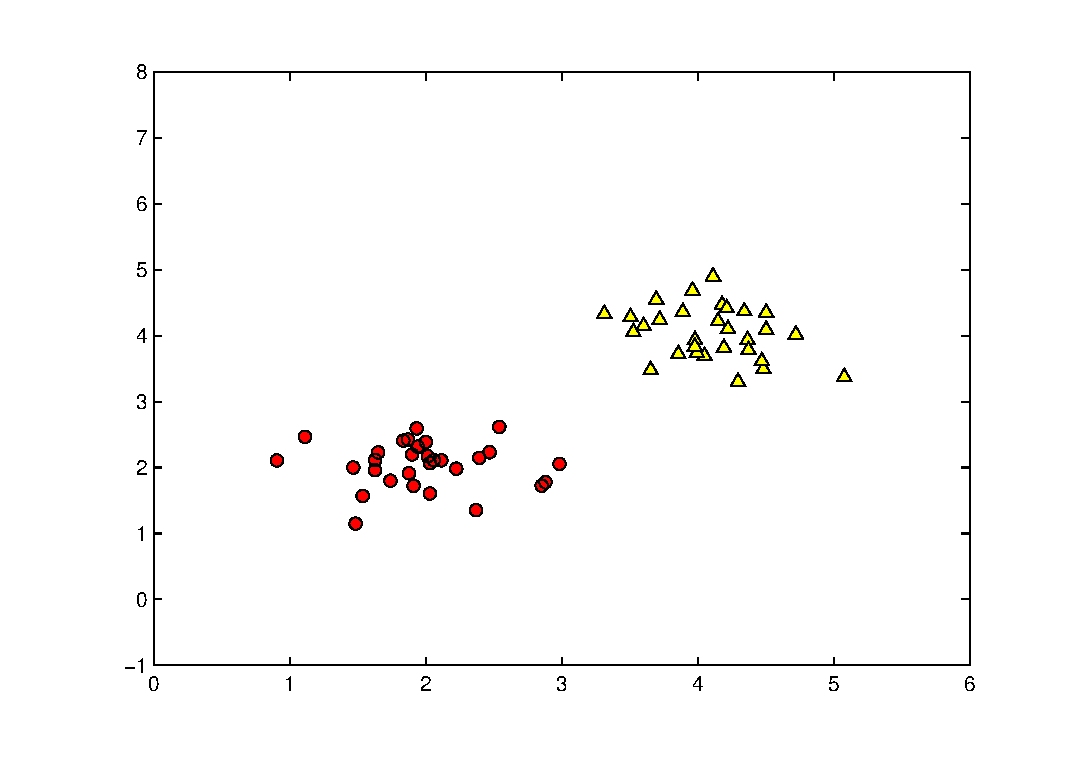
\includegraphics[width=.9\textwidth]{figures/dataset.eps}
    \end{figure}
\end{frame}

\begin{frame}[fragile]{SVM Primal Problem}
    \begin{minted}[fontsize=\scriptsize]{matlab}
function [w, b] = svm_primal(X, Y)

[m, n] = size(X);
%% SVM formulation
cvx_begin
    variables w(1,n) b(1)
    minimize(pow_pos(norm(w, 2), 2))
    - Y .* (X * w' + ones(m,1)*b) + ones(m,1) <= zeros(m,1);
cvx_end
    \end{minted}
\end{frame}


\begin{frame}[fragile]{SVM Dual Problem}
    \begin{minted}[fontsize=\scriptsize]{matlab}
function [w, b] = svm_lagrangian(X, Y)

[m, n] = size(X);
%% Dual problem of the Lagrangian formulation.
Z = repmat(Y, 1, n) .* X;
H = Z * Z'; % MxM matrix
cvx_begin
    variables lambda(m, 1)
    %maximize ( sum(lambda) - .5 * lambda' * H * lambda )
    maximize ( sum(lambda) - .5 * quad_form(lambda, H) )
    lambda'*Y == 0;
    lambda >= zeros(m, 1);
cvx_end

% w is 1xN
w = (lambda .* Y)' * X;
% Non-zero lagrangian multipliers.
l1 = find(lambda > 1e-6 & Y == 1);
l2 = find(lambda > 1e-6 & Y == -1);
% b calculation as Gunn1998 suggested.
b = - .5 * w * (X(l1(1), :) + X(l2(1), :))';
    \end{minted}
\end{frame}

\begin{frame}{Problem Solution}
    \begin{figure}[!htb]
        \centering
        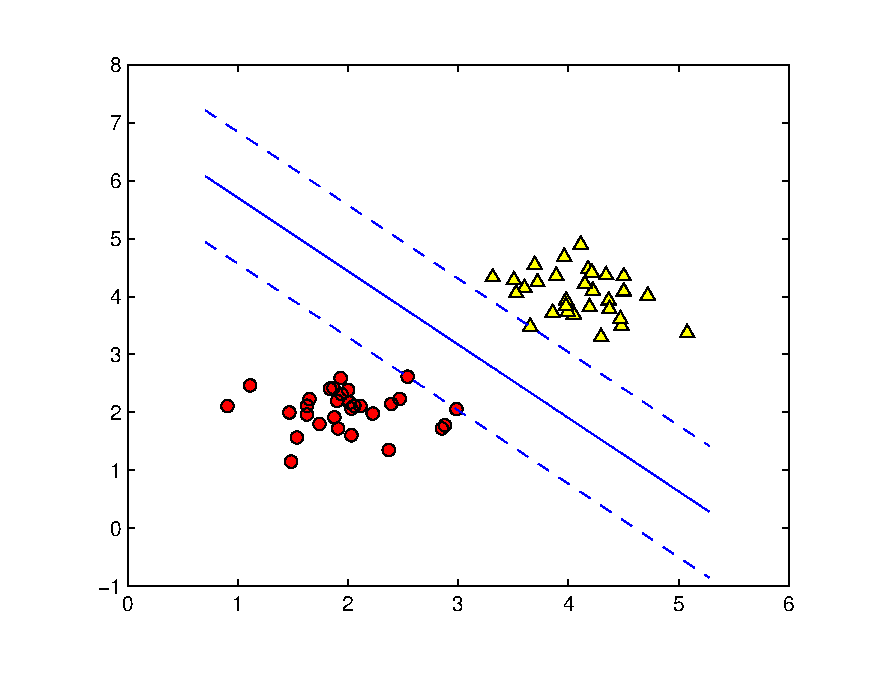
\includegraphics[width=.9\textwidth]{figures/solution.eps}
    \end{figure}
\end{frame}

\begin{frame}[fragile]
    \scriptsize
    \begin{verbatim}
-------------------------------------------------------------------
 number of iterations   = 22
 primal objective value = -2.01515477e+00
 dual   objective value = -2.01515479e+00
 gap := trace(XZ)       = 1.58e-08
 relative gap           = 3.13e-09
 actual relative gap    = 3.13e-09
 rel. primal infeas     = 2.76e-12
 rel. dual   infeas     = 1.00e-12
 Total CPU time (secs)  = 0.61  
 CPU time per iteration = 0.03  
 termination code       =  0
-------------------------------------------------------------------
 number of iterations   = 14
 primal objective value = -1.00757737e+00
 dual   objective value = -1.00757740e+00
 gap := trace(XZ)       = 3.09e-08
 relative gap           = 1.02e-08
 actual relative gap    = 1.02e-08
 rel. primal infeas     = 1.56e-12
 rel. dual   infeas     = 1.01e-12
 Total CPU time (secs)  = 0.20  
 CPU time per iteration = 0.01  
 termination code       =  0
-------------------------------------------------------------------
    \end{verbatim}
    
    
\end{frame}


\section{Conclusions}

\begin{frame}{Conclusions}
    \begin{itemize}
        \item SVM is a famous technique for classification problems
        \item The SVM problem consists in looking for separating hyperplane with the
            largest margins 
        \item It leads to a convex problem 
        \item There are advantages in using the Lagrangian formulation 
        \item The solution of the dual problem is optimal (KKT conditions)
        \item With a little modification, the presented formulation can handle more
            complex problems
    \end{itemize}
    
\end{frame}




\begin{frame}{Further Reading}
    \bibliographystyle{apalike}
    \bibliography{references}
\end{frame}

\end{document}
